\documentclass{VUMIFPSkursinis}
\usepackage{algorithmicx}
\usepackage{algorithm}
\usepackage{algpseudocode}
\usepackage{amsfonts}
\usepackage{amsmath}
\usepackage{bm}
\usepackage{caption}
\usepackage{color}
\usepackage{float}
\usepackage{graphicx}
\usepackage{listings}
\usepackage{subfig}
\usepackage{wrapfig}

% Titulinio aprašas
\university{Vilniaus universitetas}
\faculty{Matematikos ir informatikos fakultetas}
\department{Programų sistemų katedra}
\papertype{Kursinis darbas}
\title{Krepšinio taisyklių pažeidimo aptikimas}
\titleineng{Recognizing Violations of Basketball Rules using Computer Vision}
\status{3 kurso 6 grupės studentas}
\author{Lukas Cedronas}
% \secondauthor{Vardonis Pavardonis}   % Pridėti antrą autorių
\supervisor{partn. prof. dr. Vytautas Ašeris}
\date{Vilnius – \the\year}

% Nustatymai
% \setmainfont{Palemonas}   % Pakeisti teksto šriftą į Palemonas (turi būti įdiegtas sistemoje)
\bibliography{bibliografija}

\begin{document}
\maketitle

\tableofcontents

\sectionnonum{Įvadas}
Krepšinio dinamiškumas, intensyvumas ir populiarumas lemia tai, jog teisėjų priimami sprendimai gali būti šališki \cite{ProfitableBias} arba, dėl tokių faktorių kaip nuovargis, prastai pagrįsti \cite{MissedCalls}. Norint išvengti žmogiškųjų klaidų ir teisėjavimą padaryti objektyvesniu, į pagalbą galima pasitelkti kompiuterines technologijas. Technologijos, skirtos žaidimo įrašymui realiu laiku ir prieigai prie nufilmuotos medžiagos žaidimo metu teisėjų naudojama jau nuo seno, tačiau sritis, kurioje krepšinis dar nėra pažengęs, bet iš kurios galėtų gauti nemažai naudos – kompiuterinė rega (\textit{angl.} computer vision). Pasitelkus priemones, skirtas vaizdo apdorojimui, analizei ir automatizuotam sprendimų priėmimui galima iki tam tikro laipsnio teisėjavimo naštą perkelti kompiuteriui. Kompiuterio pagalba sporte ar sporto teisėjavime nėra naujiena – technologijų sėkmę gali paliudyti  2018 m. FIFA pasaulio čempionate naudotas Video Assistant Referee, peržiūrintis ir įvertinantis teisėjo padarytą nuosprendį. Tačiau nepaisant to, ši sritis nėra pakankamai pažengusi, kad visiškai pakeistų teisėjus. Bet kokiai programinei įrangai išanalizuoti vaizdo įrašą ir prieiti prie teisingo sprendimo trukdo tokie faktoriai kaip vaizdo kokybė, pasirinktas kameros kampas, judančių objektų susiliejimas, žaidėjų bei kamuolio spalvų panašumas, objektų smulkumas. Tad siekiant išbandyti pačio atpažinimo algoritmo efektyvumą kiek galima labiau atsiribojant nuo techninių kliūčių, šiame darbe bus naudojama vaizdinė medžiaga, kur:
\begin{itemize}
 \item Tarp fono, žaidėjo ir kamuolio turi būti kiek galima didesnis kontrastas.
 \item Kamuolio spalva – ryški, aukštas sodrumas (\textit{angl.} saturation).
 \item Fonas – šviesus, jame – kiek galima mažiau triukšmo (atpažinimui nereikalingų objektų).
 \item Žaidėjas su kamuoliu užima kiek įmanoma didesnį plotą visame kadre (tačiau vis dar privalo matytis kojos ir ranka).
 \item Kamera pastatyta prie žemės (tam, kad kuo geriau matytųsi, kaip ant paviršiaus dedama koja).
 \item Žaidėjas yra vienas.
 \item Žaidėjas dėvi ryškius batus ir pirštines.
\end{itemize}

Darbe bus išanalizuoti probleminiai faktoriai, sukeliantys trukdžių vaizdo atpažinime, pasirinktos metodikos, padedančios atpažinti kamuolio poziciją rankų atžvilgiu bei žingsnius, bei pritaikytas algoritmas atpažinti, kada pažeista žingsnių taisyklė. Darbo tikslas – sukurti programinę įrangą, gebančią atpažinti žingsnių taisyklės pažeidimą (šiame darbe bus remiamasi NBA taisyklėmis). Darbo uždaviniai:
\begin{itemize}
 \item Sukurti žingsnių bei kamuolio mušimo atpažinimo algoritmą.
 \item Remiantis skaitmeniniu vaizdo apdorojimo technologijomis algoritmą įgyvendinti.
 \item Įvertinti įgyvendintos programos efektyvumą su vaizdo medžiaga.
\end{itemize}

\section{Naudoti įrankiai ir metodai}
Šiam darbui atlikti pasirinkta Python programavimo kalba. Dėl Python paprastumo ir duomenų analizės specialistų polinkio naudoti šią kalbą internete gausu straipsnių ir kitų išteklių būtent šiai kalbai. Python leidžia susifokusuoti į aukšto lygmens abstrakcijas, kas labai praverčia kompiuterinėje regoje analizuojant ir darant operacijas su paveikslėliais, vaizdo medžiaga ir panašiai. Be to, kadangi Python yra interpretuojama programavimo kalba – jos nereikia kompiliuoti – atsiranda galimybė programuoti interaktyviai, t.y. greitai išgauti rezultatus iš įvairių skaičiavimų nevykdant iš naujo jau parašytos programos. 

Kompiuterinės regos algoritmų įgyvendinimui nagrinėtos dvi bibliotekos: SimpleCV [1] ir OpenCV [2]. OpenCV – plačiai naudojama kompiuterinės regos užduotims spręsti skirta biblioteka, kuri yra nemokama. OpenCV parašyta C++ kalba, tačiau galima naudoti OpenCV su  Python apvalku ant C++ rašyto pagrindo. Taip pasiekiamas artimas C++ efektyvumas kartu su Python kalbos paprastumu.
SimpleCV – panaši biblioteka į OpenCV, tačiau dar labiau abstrahuota, fokusas į naudojamo paprastumą, prieinamumą pradedantiesiems. Dėl medžiagos gausos ir didesnių galimybių sukurti efektyvų algoritmą nuspręsta naudoti OpenCV.

Vaizdo medžiagai išgauti naudojama Xiaomi Redmi 5 Plus kamera, gebanti filmuoti 1080p, 60 kadrų per sekundę greičiu. 
\section{Pirminis vaizdo apdorojimas}
\subsection{Kompiuterinės regos algoritmai dominančių regionų išskyrimui}
Pirmiausia vaizdas yra apdorojamas, siekiant išgauti objektus, kuriems vėliau bus pritaikomas algoritmas. Šiame darbe analizuojami svarbiausi objektai yra trys: kamuolys, žaidėjo rankos ir pėdos. Tad programą galima išskirti į dvi dalis: pirmoji – naudojantis kompiuterinės regos algoritmais išgauti šiuos tris objektus ir sąveikas tarp jų, ir antroji – su gauta informacija atlikti žingsnius, aprašytus taisyklės pažeidimo algoritme. 

Galima pamanyti, jog užtenka atrasti apvalų objektą ir teigti, jog tai – kamuolys, tačiau reikia atsižvelgti į tai, kad: 
\begin{enumerate}
\item Negalima garantuoti, kad kamuolys yra vienintelis apvalus objektas kadre. Pavyzdžiui, į kadrą gali patekti žaidėjo galva, arba pėda gali būti pastatyta taip, jog algoritmas ją irgi palaikys apvaliu objektu. 
\item Net jei ir užtikriname, kad kamuolys – vienintelis apvalus objektas kadre, judėdamas jis tampa nebe toks apvalus. Jei kameros kokybė prastesnė, greitai judantis objektas gali tapti išsiliejęs ir ištemptas.
\end{enumerate}
\subsection{Segmentavimas}
Aukščiau išvardintų problemų sprendimui pasirinktas segmentavimo pagal spalvą metodas. Segmentavimas – procesas, kai vaizdas yra suskirstomas į nesikertančius regionus \cite{ImageSegmTech}. Tad segmentuojant pagal spalvą išskiriamas regionas, atitinkantis kamuolio vietą kadre, su prielaida, kad kamuolys bus kitokios, iš anksto apibrėžtos spalvos, negu bet kas kitas kadre. Šitaip programa galės nesunkiai išskirti kamuolį kaip atskirą objektą. 

Jei kamuolio spalva nėra pakankamai ryški ir išsiskirianti iš fono, minėtu metodu atpažinti kamuolį darosi sunku, todėl kamuolio spalva turi būti kiek galima sodresnė. Taip pat naudojamas HSV modelis, kuris padeda dalinai išspręsti šią problemą \cite{StaloTenisas}: pasinaudojus HSV modeliu, atpažinti kamuolį darosi lengviau, net jei kinta apšvietimas, kadangi spalva išlieka ta pati, keičiasi tik sodrumas kartu su šviesumu. Tačiau reikia atkreipti dėmesį, jog OpenCV naudojama spalvos skalė skiriasi nuo įprastos. Spalvos atspalvis (\textit{angl.} hue) išreiškiamas laipsniais nuo 0 iki 360, tačiau OpenCV kiekvienai reikšmei naudoja 8 bitų dydžio char reprezentaciją, todėl galimų reikšmių intervalas yra [0; 255]. Tad būtina atspalvio reikšmes normalizuoti (t.y. padalinti iš dviejų), prieš jas panaudojant OpenCV kontekste. Šiame darbe minint HSV reikšmes atspalviui bus naudojamas standartinis laipsnių modelis.

Taisyklės pažeidimo algoritmui reikia žinoti, kada kamuolys yra rankoje. Tačiau vykdant spalvos segmentavimą išskirti tik ranką yra beveik neįmanoma, jei rankos spalva sutampa su kitų elementų, esančių kadre, spalva – pavyzdžiui, žaidėjo odos. Tokiu atveju išskirti ranką kaip objektą yra keletas būdų – pavyzdžiui, Haar kaskadų metodas, paremtas kompiuterio mokymo principais: su pozityviais paveikslėliais (šiuo atveju tai būtų paveikslėlis, kuriame pavaizduota ranka) ir negatyviais (tai paveikslėliai, kurie nėra ranka) sukuriama atpažinimo formulė. \cite{HaarCascades}  Tačiau toks rankų atpažinimo metodas gana sudėtingas ir lėtas, todėl nuspręsta imtis kitos išeities – užsidėti pirštinę, kurios spalva būtų unikali visame kadre. Spalva pasirinkta geltona, jos atspalvio kodas svyruoja nuo 96 iki 112. Pasirinkus platesnį intervalą pradedami segmentuoti šalutiniai objektai, siauresnį - rankos regione atsiranda dėmės, kadangi ne visos spalvos būna rastos. Tokie patys principai pritaikomi ir pėdų bei kamuolio radimui.
\begin{figure}[H]
	\centering
	
\includegraphics[scale=1]{imgs/rank}
	\caption{Rankos prieš segmentavimą.}
	\label{imgs:rank}
\end{figure}
\begin{figure}[H]
	\centering
	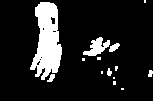
\includegraphics[scale=1]{imgs/segrank}
	\caption{Rankos po segmentavimo. Dešinėje pusėje matyti šiek tiek triukšmo, kuris bus pašalintas atliekant eroziją.}
	\label{imgs:segrank}
\end{figure}
\subsection{Morfologinės transformacijos}
Po segmentavimo išskirtas objektas gali turėti triukšmo (t.y. nereikalingų dėmių, smulkių objektų fone ) (2 pav.). Tam, kad jų nebeliktų, pritaikomos morfologinės transformacijos: erozija ir plėstis. Erozija – procedūra vykdoma ant matricos (paveikslėlio reprezentacijos). Turėdami dvi matricas -  matricą A ir matricą B (vadinamą struktūriniu elementu) – galime praeiti su struktūriniu elementu pro kiekvieną matricos A reikšmę, atliekant sankirtą su visom struktūrinio elemento reikšmėm ir tomis, kurias B “apglėbia” A matricoje. Formaliai tai užsirašo šitaip \cite{ImageAnalysisMorph}:

\begin{equation}\label{eq:erozija}
A \ominus B = \bigcap_ {b \in B } (A)_{-b} .
\end{equation}

Po erozijos paveikslėlyje ne tik sumažėja triukšmo, bet ir sumažėja pavaizduoto objekto plotas. Todėl panaudojama plėstis, kuri gali būti naudojama kaip priešinga operacija erozijai: po plėsties objekto plotas išdidinamas. Kaip ir erozijos atveju, naudojamas struktūrinis elementas, tik šį kartą vietoje sankirtos naudojama sąjunga \cite{ImageAnalysisMorph}:

\begin{equation}\label{eq:plestis}
A \oplus B = \bigcup_ {b \in B } (A)_{b} .
\end{equation}

Svarbu plėstį atlikti po erozijos, priešingu atveju plėstis išryškins triukšmą (mažus objektus padarys didesniais), o erozija juos vėl apmažins – galutiniame variante gaunama kažkas panašaus į originalą. Pirma vykdant eroziją, o tik vėliau plėstį užtikriname, kad bus panaikintas triukšmas, o svarbūs objektai nepraras savo ploto. 

OpenCV leidžia pasirinkti, kiek iteracijų norima atlikti. Kadangi po segmentacijos išlaikyti objekto formą nėra svarbu (pavyzdžiui, objektų atpažinimas nenukentės, jeigu nebus galima atskirti rankos pirštų), plėstis atliekama daugiau kartų, nei buvo atlikta erozija. Šitaip galime išgauti objektus, kurių plotas yra didesnis, nei originalo. Tai itin svarbu segmentuojant pėdas, kadangi 3.2. poskyryje aprašytas algoritmas žingsnį atpažins pagal tai, ar pėdų regionai persiklojo vienas su kitu. Padidinus plotą sumažėja rizika, žingsnis nebus aptiktas.
\begin{figure}[H]
	\centering
	
\includegraphics[scale=1]{imgs/morphrank}
	\caption{Rankos atlikus morfologines operacijas. Triukšmas buvo pašalintas, o rankų užimamas plotas - padidėjo.}
	\label{imgs:morphrank}
\end{figure}
\subsection{Kontūrų radimas ir užpildymas}
Išgavus regionus, kurie atitinka taisyklės pažeidimo atpažinimo algoritmui reikalingus objektus - ranką, kamuolį bei pėdą - vykdomas sekantis žingsnis: kontūrų radimas bei jų užpildymas. Kadangi po segmentacijos jokie regionai nepersikloja vienas su kitu, iš segmentuotų regionų negalima gauti jokios informacijos apie tai, ar iš tiesų žaidėjas rankomis liečia kamuolį. Reikalingas dar vienas žingsnis - rasti pilną kamuolio regioną, įskaitant ir tą dalį, kurią uždengia ranka. Tam pasitelkiamas mažiausio apskritimo radimo algoritmas, padedantis atkurti pilnus kamuolio kontūrus. OpenCV apskritimo kontūrui atrasti naudoja Emo Welzl algoritmą, kuris nepriklausomai nuo regiono, apskritimo kontūrą randa tiesiniu laiku \cite{smallestenclosing}. Algoritmo principas - ant pradinės taškų aibės užbrėžti mažiausią apskritimą, kuriame yra visi šie taškai, bei pasirinkus kitą atsitiktinį tašką apskritimą didinti: \cite{smallestenclosing}
\begin{figure}[H]
	\centering
	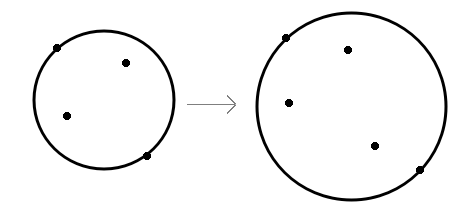
\includegraphics[scale=1]{imgs/welzl}
	\caption{Welzl algoritmo supaprastinimas.}
	\label{imgs:welzl}
\end{figure}
Tačiau apskritimo radimas yra jautrus segmentavimo metu atsiradusiam triukšmui: jeigu po kamuolio segmentacijos fone dar lieka pašalinių objektų, panašių į apskritimą, jie gali būti aptinkami algoritmo vietoje kamuolio. Todėl būtina prieš tai atsirinkti didžiausią regioną, ant kurio bus vykdomas algoritmas - mažai tikėtina, kad triuškmas galėtų sugeneruoti objektą, didesnį už kamuolį.
Kontūrai vėliau užpildomi, rezultate gaunant visą plotą, kuriame yra kamuolys, net jei jis ir uždengtas kitų objektų.
\begin{figure}[H]
	\centering
	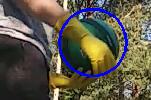
\includegraphics[scale=1]{imgs/kamuol}
	\caption{Kamuolio kontūrai, apibrėžti aplink patį kamuolį. Kontūrai - vientisas apskritimas, nepaisant to, jog didelę kamuolio dalį dengia ranka.}
	\label{imgs:kamuol}
\end{figure}
\section{Objektų ir jų padėties atpažinimo algoritmas}
Čia aprašomas objektų padėties atpažinimas bei apibendrintas algoritmas, kaip iš vaizdo gaunama reikiama informacija apie tai, ar kamuolys rankose bei  atliktas žingsnis.
\subsection{Rankos, kamuolio, pėdų  atpažinimas ir tarpusavio sąryšiai}
Atlikus segmentavimą, morfologines transformacijas bei kontūrų užpildymą, turima pakankamai informacijos teiginių apie objektų tarpusavio sąryšius konstravimui.
OpenCV visus paveikslėlius galima reprezentuoti loginėmis matricomis. Tad ranka, kamuolys bei pėdos saugomi kaip loginės matricos, kas įgalina efektyviai atlikti logines operacijas.
\subsection{Algoritmas}
Aukščiau aprašytas procedūras galima apibendrintai aprašyti algoritmu, kuriuo vadovaujasi ir sukurta programinė įranga.
\begin{enumerate}
	\item Vaizdo medžiaga išskiriama į kadrus.  
	\item Kiekvienam kadrui vykdoma segmentacija pagal iš anksto numatytas spalvas, gaunami regionai. 
	\item Regionams vykdomos morfologinės, kontūro radimo operacijos.
	\item Kontūrai užpildomi.
	\item Persidengiantys regionai konvertuojami į logines matricas, atliekamos Būlio disjunkcijos.
\end{enumerate}

Disjunkciją atlikus su kamuolio ir rankos matricomis, gaunama nauja matrica, kurioje teigiama reikšmė (1) reiškia tai, jog šioje vietoje ranka ir kamuolys persidengia. Jeigu matricoje teigiamų reikšmių lyginant su visomis reikšmėmis yra daugiau, negu numatytas santykis, kamuolys yra rankoje. Kamuolio buvimo rankoje būsena yra saugoma atminty sulyg kiekvienu kadru.


Žingsnio išgavimo technika šiek tiek skiriasi. Paeksperimentavus su filmuota medžiaga nuspręsta, jog žemės segmentavimas nėra efektyvus: pilkšva aikštelių spalva atsikartoja daug kur - drabužiuose, fone. Vietoje to suskaičiuojamas pėdų kontūrų kiekis. Jeigu pėdos toli viena nuo kitos - kontūrų atitinkamai bus rasta du. Kita vertus, atliekant žingsnio judesį, kojos visada persidengs viena su kita. Todėl daroma prielaida, jog kiekvieno žingsnio eigoje pėdos taip pat persidengs. Po segmentavimo ir diliacijos, persidengiančių pėdų regionai sudaro vientisą aibę, kuri savo ruožtu turi vienintelį kontūrą. Jei vaizdo apdorojimo eigoje aptinkama, jog pėdų segmentų skaičius iš dviejų tapo vienu, programa nuspręs, jog buvo padarytas žingsnis. 

\section{Taisyklės pažeidimo atpažinimas}
Šiame darbe nagrinėjama taisyklė yra oficialiame NBA puslapyje aprašytos 10 taisyklės 14 skyriuje. Taisyklė sako, jog gavęs kamuolį, žaidėjas gali padaryti daugiausiai du žingsnius prieš kamuolį išmesdamas ar atiduodamas kitam žaidėjui. 

Taisyklė laikoma pažeista, jeigu tenkinama ši sąlyga:  tuo metu, kol kamuolys laikomas rankose, užfiksuojami daugiau negu du žingsniai. Programa saugo būseną, kada kamuolys yra laikomas rankose, tad tai, jog žaidėjas žingsnius turi padėjo daugiau nei žingsnius tame laiko intervale leidžia daryti išvadą, kamuolio mušinėjimo veiksmas yra sustabdytas - kitaip vargu, ar žaidėjas būtų spėjęs padaryti daugiau nei du žingsnius. 


\sectionnonum{Rezultatai ir išvados}
Rezultatų ir išvadų dalyje turi būti aiškiai išdėstomi pagrindiniai darbo
rezultatai (kažkas išanalizuota, kažkas sukurta, kažkas įdiegta) ir pateikiamos
išvados (daromi nagrinėtų problemų sprendimo metodų palyginimai, teikiamos
rekomendacijos, akcentuojamos naujovės).

\printbibliography[heading=bibintoc]  % Šaltinių sąraše nurodoma panaudota
% literatūra, kitokie šaltiniai. Abėcėlės tvarka išdėstomi darbe panaudotų
% (cituotų, perfrazuotų ar bent paminėtų) mokslo leidinių, kitokių publikacijų
% bibliografiniai aprašai.  Šaltinių sąrašas spausdinamas iš naujo puslapio.
% Aprašai pateikiami netransliteruoti. Šaltinių sąraše negali būti tokių
% šaltinių, kurie nebuvo paminėti tekste.

\appendix  % Priedai
\section{Nuoroda į GitHub}
\url{https://github.com/LukasCed/basketball-rule-violation-recognition}

\end{document}
